\subsection{RQ3: To what extent can specialized SLMs improve the detection of errors in generated code?}
\label{sec:rq3}

The four specialized detectors are compared with their Gemma 4 E4B base model. Table~\ref{tab:rq3_specialization} summarizes Accuracy and Macro-F1 under the paired comparison used for this analysis. Values in parentheses report the difference in percentage points relative to the base model. The paired values can differ slightly from the standalone results in Table~\ref{tab:rq2_detection} because this comparison uses only rows available for both the base and specialized conditions.

\newcommand{\improvedcell}[1]{\cellcolor{green!20}#1}
\newcommand{\worsecell}[1]{\cellcolor{red!20}#1}
\newcommand{\uncertaincell}[1]{\cellcolor{gray!15}#1}

\begin{table}[htbp]
\centering
\caption{Performance of the specialized detectors relative to the Gemma 4 E4B base model. The base reaches 45.9\% Accuracy and 37.1\% Macro-F1 on the paired subset. Values in parentheses indicate the difference in percentage points. Green cells indicate improvements whose paired bootstrap interval excludes zero, while gray cells indicate differences whose interval includes zero.}
\label{tab:rq3_specialization}
\begin{tabular}{lrr}
\toprule
\textbf{Specialized Model} &
\textbf{Accuracy} &
\textbf{Macro-F1} \\
\midrule

Best Acc
& \improvedcell{77.9 (+32.0)}
& \improvedcell{51.0 (+13.9)}
\\

Weighted MF1
& \improvedcell{73.6 (+27.7)}
& \improvedcell{54.3 (+17.2)}
\\

Balanced Acc
& \improvedcell{67.9 (+22.0)}
& \uncertaincell{38.1 (+1.0)}
\\

Balanced MF1
& \improvedcell{63.8 (+17.9)}
& \uncertaincell{36.0 (-1.1)}
\\

\bottomrule
\end{tabular}
\end{table}

All four specialized configurations increase Accuracy relative to the base model, but their effects on Macro-F1 differ substantially. Best Acc produces the largest Accuracy improvement, increasing the metric by 32.0 percentage points, with a paired task-level bootstrap interval of [25.0, 39.2]. Its Macro-F1 also increases by 13.9 points, with an interval of [6.7, 21.0]. Weighted MF1 produces a slightly smaller Accuracy gain of 27.7 points [21.3, 34.2], but the largest Macro-F1 improvement, increasing it by 17.2 points [11.9, 22.3]. These results show that specialization improves detection under both optimization objectives, while the objective determines which aspect of performance benefits most strongly.

\begin{figure}[htbp]
\centering
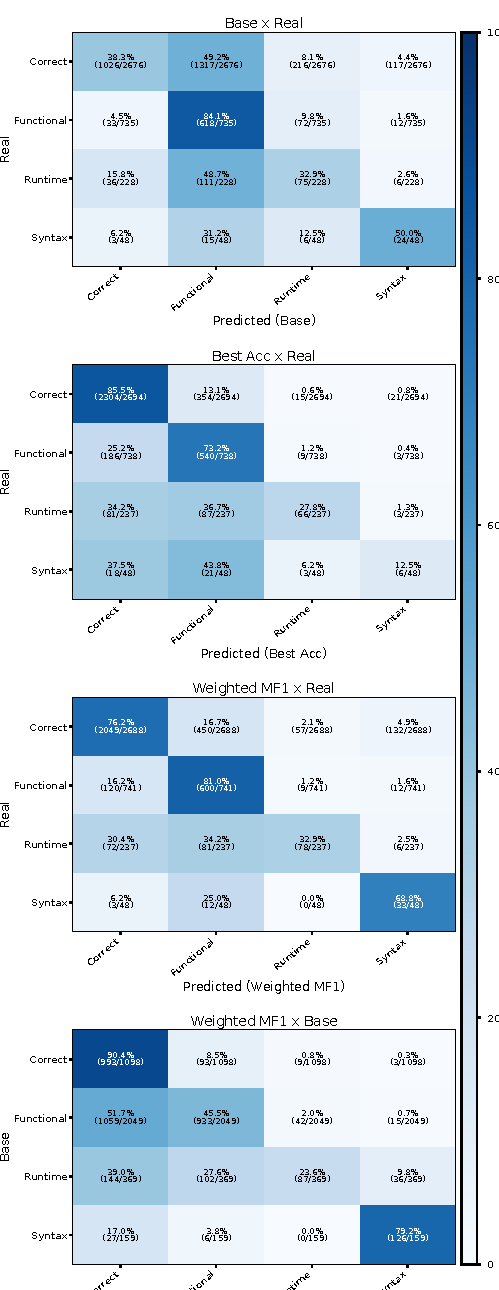
\includegraphics[width=\columnwidth]{figures/confusion_matrices.pdf}
\caption{Row-normalized confusion matrices under a primary-label reduction with priority Syntax, Runtime, Functional, and Correct. Each cell reports the proportion and the counts as predicted/reference total. The first three matrices compare the base, Best Acc, and Weighted MF1 predictions with the execution-derived reference. The last matrix compares Weighted MF1 predictions directly with those of the base model. Unparseable outputs are excluded only from this primary-label visualization.}
\label{fig:confusion}
\end{figure}

The Accuracy-oriented detector achieves its improvement primarily by becoming substantially more likely to predict \emph{Correct}. Figure~\ref{fig:confusion} shows that, for the base model, only 38.3\% of samples whose primary reference label is Correct are predicted as Correct, while 49.2\% are predicted as Functional. After Accuracy-oriented specialization, Correct-to-Functional confusion decreases to 13.1\%, while Correct predictions increase substantially. However, this shift also affects the error classes. Functional-to-Correct increases from 4.5\% to 25.2\%, Runtime-to-Correct from 15.8\% to 34.2\%, and Syntax-to-Correct from 6.2\% to 37.5\%. Thus, the Accuracy gain is accompanied by a stronger tendency to predict the dominant Correct outcome.

The Macro-F1-oriented detector exhibits a different behavior. In the full multilabel evaluation reported in Table~\ref{tab:rq2_detection}, Best Acc reaches 77.8\% Accuracy and 50.9\% Macro-F1, whereas Weighted MF1 reaches 73.5\% Accuracy and 54.2\% Macro-F1. The difference is also visible at the class level. Best Acc obtains 85.3\% Correct Recall, 69.1\% Functional Recall, 27.8\% Runtime Recall, and 11.8\% Syntax Recall. Weighted MF1 reduces Correct Recall to 75.9\%, but increases Functional Recall to 77.9\%, Runtime Recall to 32.9\%, and Syntax Recall to 64.7\%. The Macro-F1-oriented objective therefore sacrifices part of the strong preference for Correct in exchange for a more balanced error-detection profile.

The confusion matrices reinforce this difference. Relative to Best Acc, Weighted MF1 reduces Functional-to-Correct confusion from 25.2\% to 16.2\% and Syntax-to-Correct confusion from 37.5\% to 6.2\%. The improvement is especially pronounced for \emph{Syntax Error}, whose recall increases from 11.8\% under Best Acc to 64.7\% under Weighted MF1. This result shows that the training objective changes not only the aggregate score but also which types of errors the specialized detector is able to recognize.

\emph{Runtime Error} remains the most difficult category after specialization. Weighted MF1 reaches 32.9\% Runtime Recall, which is higher than Best Acc at 27.8\%, but still considerably below its recall for Functional and Syntax Errors. The primary-label matrices similarly show substantial confusion between Runtime, Functional, and Correct predictions. Specialization therefore changes how Runtime cases are distributed among predictions, but does not eliminate the difficulty of identifying this error category.

The explicitly balanced training strategies produce a different result. Balanced Acc increases Accuracy by 22.0 percentage points relative to the base, with a paired bootstrap interval of [15.0, 29.1], while Balanced MF1 increases it by 17.9 points [11.4, 24.5]. Their Macro-F1 changes, however, are much smaller. Balanced Acc changes Macro-F1 by +1.0 point, with an interval of [-4.6, 6.6], while Balanced MF1 changes it by -1.1 points, with an interval of [-6.5, 4.4]. The intervals therefore include zero for both balanced configurations, and the observed differences do not provide clear evidence of a Macro-F1 improvement over the base model.

The class-level results help explain this behavior. Balanced Acc reaches 74.4\% Correct Recall and 65.8\% Functional Recall, but only 15.2\% Runtime Recall. Balanced MF1 reaches 68.6\% Correct Recall, 65.8\% Functional Recall, and 13.9\% Runtime Recall. Both configurations obtain 0\% Syntax Recall. As described in the experimental setup, Syntax examples were excluded from balanced training because of their low representation and the availability of deterministic compilation for this outcome. The unchanged validation and test partitions preserve these cases during evaluation, making the loss of Syntax detection directly observable.

The final matrix in Figure~\ref{fig:confusion} further illustrates that specialization changes prediction behavior rather than simply correcting every previous decision. Among samples predicted as Correct by the base model, 90.4\% remain Correct under Weighted MF1. In contrast, only 23.6\% of samples previously predicted as Runtime remain Runtime, while 51.7\% of samples previously predicted as Functional are reclassified as Correct. These transitions do not indicate correctness by themselves because the matrix compares two sets of predictions rather than predictions against the reference. Instead, they illustrate how strongly fine-tuning changes the detector's decision boundaries.

Overall, specialization improves error detection, but the benefits depend on the optimization objective. Accuracy-oriented training produces the largest gain in exact-set Accuracy and shifts the detector toward recognizing \emph{Correct}, whereas Macro-F1-oriented training yields the largest improvement in Macro-F1 and a more balanced profile across the error categories. The evaluated balancing strategies also increase Accuracy relative to the base model, but do not produce a clear Macro-F1 improvement. Across all specialized configurations, \emph{Runtime Error} remains the most difficult outcome, indicating that specialization improves the detector substantially without eliminating the main class-specific limitation observed in the general-purpose models.